% !TeX spellcheck = en_GB
\documentclass[a4paper, 12pt]{scrartcl}

\setkomafont{title}{\rmfamily}
\addtokomafont{disposition}{\rmfamily}

\usepackage[english]{babel}
\usepackage[T1]{fontenc}
\usepackage{lmodern}
\usepackage[utf8]{inputenc}

\usepackage{amsmath}
\usepackage{amssymb}
\usepackage{amsfonts}
\usepackage{amsthm}

\usepackage{hyperref}
\usepackage{listings}
\usepackage{color}

\usepackage{appendix}

\definecolor{codegreen}{rgb}{0,0.6,0}
\definecolor{codegray}{rgb}{0.5,0.5,0.5}
\definecolor{codepurple}{rgb}{0.58,0,0.82}
\definecolor{backcolour}{rgb}{0.95,0.95,0.92}

\lstdefinestyle{mystyle}{
	backgroundcolor=\color{backcolour},   
	commentstyle=\color{codegreen},
	keywordstyle=\color{magenta},
	numberstyle=\tiny\color{codegray},
	stringstyle=\color{codepurple},
	basicstyle=\footnotesize\ttfamily,
	breakatwhitespace=true,         
	breaklines=true,                 
	captionpos=b,                    
	keepspaces=true,                 
	numbers=left,                    
	numbersep=5pt,                  
	showspaces=false,                
	showstringspaces=false,
	showtabs=false,                  
	tabsize=2
}

\lstset{style=mystyle}
\usepackage{icomma}

\usepackage{graphicx}
\usepackage{subcaption}

\usepackage{enumitem}

\usepackage{placeins}
%opening
\title{{\large \textbf{Introduction to Stochastic Demography Project}}\\
{\Large \textbf{Forecasting the Total Fertility Rate in some European countries}}}
\author{{\large Oscar Granlund}\\
{\large 37920}}
\date{}

\begin{document}

\maketitle


\section{Introduction}
In this project we try to find an autoregressive integrated moving average (ARIMA) model for forecasting the Total Fertility Rates (TFR) in 8 different European countries.
The aim is to find one (hopefully relatively simple) model that as accurately as possible forecasts the TFR in all the countries.

Accurately forecasting the Total Fertility Rate can be important for a variety of reasons, for example in some countries where birth rates are decreasing there are problems where there number of workers per retiree is decreasing and thus the workers have to contribute more; in order to accurately say how much more each worker has to pay, the forecasts of the future number of workers need to be accurate.
Since pension schemes are often regulated by governments in some way, decisions on changes are often made into political questions and thus the decision to use a particular model for forecasting birth rates are often politically charged and thus simpler models are favoured.

One could also argue that there are underlying factors that determine the TFR but such models will not be considered.
This choice was made since accurate data for latent factors can be difficult to find while many countries publish relatively accurate data for the TFR and these datasets can easily be found aggregated at \cite{web:TFR}.

\section{Autoregressive Integrated Moving Average models}
There are many approaches for analysing and forecasting time series but the two most popular approaches are exponential smoothing and autoregressive integrated moving average (ARIMA) models \cite{web:fpp}.
Exponential smoothing models are based on the trends and seasonality of the data ARIMA models try to describe the autocorrelations of the data.
For our purposes we will consider only the ARIMA family of models since in some cases choosing an ARIMA model can be interpreted as determining what random process has generated the time series.

\subsection{Autoregressive models}
An autoregressive (AR) model is where the forecast for the value of the next point is a linear combination of the values of the past points or in other words, the time series is a linear regression of itself or auto(self)-regressive(regression).
Mathematically we write the forecasted value $y_t$ in the following way:
\begin{equation*}
	y_t = \phi_0 + \phi_1y_{t-1} + \phi_2y_{t-2}+\dots+\phi_py_{t-p}+\varepsilon_t
\end{equation*}
where $p$ is the order of autoregression and $\varepsilon_t$ is an error term ( some random variable).

The optimal model (in terms of minimizing the sum of the squared residuals) can be found by defining the following vectors and matrices
\begin{equation*}
	\mathbf{y}=\begin{bmatrix}
	y_N\\
	y_{N-1}\\
	\vdots\\
	y_{p+2}\\
	y_{p+1}
	\end{bmatrix},\quad \mathbf{X}=\begin{bmatrix}
	1 & y_{N-1} & y_{N-2} & \cdots & y_{N-p+1}& y_{N-p}\\
	1 & y_{N-2} & y_{N-3} & \cdots & y_{N-p}& y_{N-p-1}\\
	\vdots& \vdots &	  & 	   &		& \vdots\\
	1 & y_{p+1} & y_{p} & \cdots & y_{3}& y_{2}\\
	1 & y_{p} & y_{p-1} & \cdots & y_{2}& y_{1}
	\end{bmatrix}
\end{equation*}
and solving the equation $\mathbf{y}=\mathbf{X}\boldsymbol{\phi}$ for the least-squares solution (with respect to $\boldsymbol{\phi}$) $\boldsymbol{\phi}=\left(\mathbf{X}^\intercal\mathbf{X}\right)^{-1}\mathbf{X}^\intercal\mathbf{y}$.
Note the absence of the first $p$ $y_t$:terms in the vector $\mathbf{y}$ and the absence of the $y_N$ term in the matrix $\mathbf{X}$, clearly we might not be using all the information known to us using this solution.
For example all $N$ datapoints can be used to determine the coefficient $\phi_0$ (the intercept or mean level).

We might also need to impose restrictions on the coefficients $\phi_i$ if we assume additional things about the underlying data, for example if we assume the random process is \emph{stationary} we need to impose the constraint $-1<\phi_1<1$ for an autoregressive model of order 1 (AR(1) model).
Because of this the naive ordinary least squares solution is usually not used, instead a system of equations called the Yule-Walker equations are solved.
The Yule-Walker equations are based upon the autocorrelations of the data.

The projection for the next datapoint $\hat{y}_{N+1}$ are given by \begin{equation*}
\hat{y}_{N+1}=\phi_0+\phi_1y_N+\phi_2y_{N-1}+\dots+\phi_{p-1}y_{N-p+2}+\phi_py_{N-p+1}
\end{equation*}
for two steps ahead we use the projected value $\hat{y}_{N+1}$ instead the observed value $y_{N+1}$ (of course, at time $N$ we don't have an observed value at for time $N+1$).
This way of projecting forwards is a commonly used technique in time series forecasting.

\subsection{Moving Average models}
The moving average (MA) model is a bit more complex than the AR models.
Here the idea is that instead of regressing on past values we regress on past forecast errors.
Mathematically we write the MA model of order $q$ (the MA($q$) model) in the following way:
\begin{equation*}
	y_t=\theta_0+\theta_1\varepsilon_{t-1}+\theta_2\varepsilon_{t-2}+\dots+\theta_q\varepsilon_{t-q}+\varepsilon_t
\end{equation*}
where the terms $\varepsilon_t$, $t=1,\dots,N$ are the errors.
Note here that the errors are not really ``observed'' in the same sense that the values $y_t$ are observed.
Instead we can get observed errors by having some forecast $\hat{y}_t$ and setting $\varepsilon_t=\hat{y}_t-y_t$.
This means that the errors depend on the forecast but the forecast also depends on the errors so a regular OLS method will not work that well.

An interesting observation is that any \emph{stationary} AR($p$) model can be written as a MA($\infty$) model.
For example an AR(1) model with $\phi_0=0$ (centred) can be written in the following way:
\begin{align*}
	y_t&=\phi_1y_{t-1}+\varepsilon_t\\
	&=\phi_1\left(\phi_1y_{t-2}+\varepsilon_{t-1}\right)+\varepsilon_t\\
	&=\phi_1^2y_{t-2}+\phi_1\varepsilon_{t-1}+\varepsilon_t\\
	&=\phi_1^2\left(\phi_1y_{t-3}+\varepsilon_{t-2}\right)+\phi_1\varepsilon_{t-1}+\varepsilon_t\\
	&=\phi^3_1y_{t-3}+\phi_1^2\varepsilon_{t-2}+\phi_1\varepsilon_{t-1}+\varepsilon_t
\end{align*}
and so on, ending up with
\begin{equation*}
	y_t=\sum_{i=0}^{\infty}\varepsilon_{t-i}\phi^i_1
\end{equation*}
which converges if $|\phi_1|<1$ which was our constraint for stationary AR(1) processes.

The converse result is true for some MA processes; in other words some MA($q$) can be written as AR($\infty$) processes.
Such processes are called invertible and they give us a way to write the current error $\varepsilon_t$ as a linear function of current and past observations $y_i$, $i=1,\dots,t$.
For a centred MA($q$) process we get
\begin{equation*}
	\varepsilon_t=\sum_{i=0}^{\infty}\left(-\theta_1\right)^iy_{t-i}
\end{equation*}
where again we need the constraint $|\theta_1|<1$.
This is the condition for a MA($q$) process being invertible.

Of course, we will never have infinitely many datapoints but the results for the infinite cases are still usable in the finite case.

\subsection{Differencing a time series and stationarity}
We have seen that a concept called stationarity seems to be important for time series forecasting so perhaps we should give a definition:

A time series $y_t$ is stationary if the properties of the time series do not change with time.
This will be the case if for all $s$, the distribution of $\left(y_t, \dots,y_{t+s}\right)$ does not depend on $t$.

Since the assumption of stationarity is so important there are techniques for transforming non-stationary time series into stationary time series.
One such technique is \emph{differencing} a time series, where we instead of considering $y_t$ consider the time series $y_t'=y_t-y_{t-1}$.

If $y_t'=y_t-y_{t-1} = \varepsilon_t$ is white noise, we have a model called the random walk model where we can write $y_t=y_{t-1} + \varepsilon_t$.
This is one of the simplest non-stationary models but still one of the most widely used ones.

If differencing once is not enough we can take the differences of the differenced time series and create the time series $y_t''=y_t'-y_{t-1}'=y_t-2y_{t-1}+y_{t-2}$.
Higher orders if differencing might also be necessary.

To describe differenced time series we often use the \emph{backshift operator} $B$.
The backshift operator $B$ is the operator such that $By_t=y_{t-1}$.
Now applying the backshift operator twice, using standard notation, we see that $B(By_t)=B^2y_t=y_{t-2}$ and we can write the first difference $y_t'=y_t-y_{t-1}$ as the operator equation $(1-B)y_t=y_t-y_{t-1}$ and similarly the second difference as $y_t''=(1-B)^2y_t=(1-2B+B^2)y_t=y_t-2y_{t-1}+y_{t-2}$.
Thus the $d$th-order difference is given by the operator $(1-B)^d$.

\subsection{The ARIMA model}
The autoregressive integrated moving average model of order ($p,~d,~q$) (ARIMA($p,~d,~q$)) is written as the following equations:

\begin{align*}
	y'_t&=c+\phi_1y_{t-1}'+\dots+\phi_py_{t-p}'+\theta_1\varepsilon_{t-1}+\dots+\theta_q\varepsilon_{t-q}+\varepsilon_t\\
	(1-B)^dy_{t}&=c+\phi_1B(1-B)^dy_{t}+\dots+\phi_pB^p(1-B)^dy_t+\theta_1B\varepsilon_t+\dots+\theta_qB^q\varepsilon_{t}+\varepsilon_t
\end{align*}
where $y'_t$ is the time series differenced $d$ times which is equal to $(1-B)^dy_{t}$.

The second equation can be rewritten by gathering all the $y_t$ terms on one side, giving:
\begin{equation*}
	\left(1-\phi_1B-\dots-\phi_pB^p\right)\left(1-B\right)^dy_t=c+\left(1+\theta_1B+\dots+\theta_qB^q\right)\varepsilon_{t}.
\end{equation*}
These equations can be interpreted as an autoregressive model plus a moving average model on a differenced time series.
The term integrated comes from the ``de-differencing'' of the estimates that we have to perform, or in other words, the summing up of the forecasted differences or if our timesteps approach zero, the integration we perform.

\subsection{Parameter selection}

Traditionally when we choose between models that are in some way nested, measures such as the Akaike information criterion (AIC), the corrected Akaike information criterion (AICc) or the Bayesian information criterion (BIC) are useful.
In this case this is however not an option since these measures of fit and complexity require that the models are fit to the same datasets which is technically not the case here since different orders of differencing $d$ change the data to be fit.
For a fixed order of differencing $d$ we can still use AIC, AICc or BIC to choose the best model so we first need to determine the order of differencing.

In order to determine the order of differencing we can use tests for stationarity (really they are called unit root tests) for many orders $d$ until we find the lowest order $d$ such that the series $(1-B)^dy$ is stationary.
There are a couple of different test for stationarity, among the most popular are the Kwiatkowski–Phillips–Schmidt–Shin (KPSS), augmented Dickey–Fuller (ADF) and Phillips–Perron (PP) tests.

Once the order of differencing $d$ has been determined, we try to determine the rest of the parameters $p$ and $q$, this can be done by fitting some initial models, selecting the best one (using AIC, AICc or BIC) and then varying $p$ and $q$ by $\pm 1$ and including/excluding the drift constant $c$.
This process of selecting the best model and searching it's ``neighbouring'' models for a better one until no new better model can be found.

Hyndman and Khandakar \cite{art:hyndkhand} suggest using the following approach for automatically fitting an ARIMA($p,~d,~q$) model to a dataset:
\begin{enumerate}
	\item Determine the order of differencing $0\leq d \leq 2$ using repeated KPSS tests.
	\item Fit 4 initial models:
	\begin{itemize}
		\item ARIMA(0, $d$, 0),
		\item ARIMA(2, $d$, 2),
		\item ARIMA(1, $d$, 0) and
		\item ARIMA(0, $d$, 1),
	\end{itemize}
	without constants if $d=2$. If $d\leq 1$ fit the previous models but also the first one again but without a constant.
	\item Select the best model of the previously fitted ones using the AICc (smallest AICc is best).
	\item Fit the new models ARIMA($p\pm1$, $d$, $q\pm1$) where $p$ and $q$ are the values that gave the previous best model. Also fit the same models including/excluding the constants.
	\item Repeat from step 2 until no better model can be found (e.g. when the same model is chosen as the best one twice in a row).
\end{enumerate}

Another approach to selecting the correct parameters (including the order of differencing) would be to have a hold-out set of the $k$ last observations (a validation set), fitting the models to only the first $N-k$ observations (a training set).
Then the forecast on the validation set and corresponding residuals can be used to chose the model ARIMA($p,~d,~q$) with lowest root mean squared residuals.
The search can be done in the same stepwise fashion as previously suggested using the RMS residuals on the validation set instead of the AICc criteria to select the best model.
In this way the order of differencing $d$ can also be selected.
A drawback is that if models are not constant throughout time then the suggested model might not be valid for future forecasts.
Another drawback is that we have less data to fit the ARIMA models to.

A third way of selecting the parameters is to look at autocorrelation and partial autocorrelation plots of the time series and using these specifying a model according to some rules.
While similar approaches can be useful confirming that a model is sound it is not very well suited for automatic model selection so we will ignore it for now.

\section{Forecasting the Total Fertility Rate in eight European countries}
For our purposes (finding one ARIMA($p,~d,~q$) model that fits many time series as well as possible) we can't really fit the models individually using the procedure suggested above.
Instead we can try something similar by trying to modify the procedure to work for multiple time series.

From \cite{web:TFR} we downloaded data for the Total Fertility Rate in 8 countries, tabulated in table \ref{tbl:countries}.
The validation set was set to be the years from 2010 onwards and the training set was set to start no earlier than 1900 (impacting only Sweden).
The countries chosen are such that they have at least 50 data points for training, also trying to sample uniformly geographically as well as ``economically''.
\begin{table}
	\centering
	\label{tbl:countries}
	\begin{tabular}{l | r r r r r r r r}
		Country & \multicolumn{1}{l}{Finland} & \multicolumn{1}{l}{Sweden} & \multicolumn{1}{l}{Estonia} & \multicolumn{1}{l}{England} & \multicolumn{1}{l}{France} & \multicolumn{1}{l}{Switzer-} & \multicolumn{1}{l}{Italy} & \multicolumn{1}{l}{Spain}\\
		& & & & \multicolumn{1}{l}{and Wales} & & \multicolumn{1}{l}{land} & & \\
		\hline
		First year & 1939 & 1891 & 1959 & 1938 & 1946 & 1932 & 1954 & 1922\\
		Last year & 2015 & 2016 & 2014 & 2014 & 2015 & 2014 & 2014 & 2014\\
		$n$ & 77 & 126 & 56 & 77 & 70 & 83 & 61 & 93
	\end{tabular}
		\caption{Table showing the countries used and the extent of their datasets.}
\end{table}

\subsection{Determining the order of differencing}
In order to determine the order of differencing we use all three tests and take the mode of their suggestions.
We also restrict the maximum number of differencing to 3 and set the $\alpha$ values of the tests to 0.05.
In listing \ref{lst:numdiffs} the code for computing the optimal number of differences for each country is shown.
Table \ref{tbl:numdiffs} shows the suggested number of differences for each country and test-type.

\begin{lstlisting}[language=R, caption={R-code for computing all suggested differences.}, label={lst:numdiffs}]
numberOfDiffs = matrix(nrow = length(countries), ncol = 3)
for (i in 1:length(countries)) {
	createAutocorrelationPlot(trainingset[[i]], countries[[i]][1]) %>%
	print()
	t   <- "level"
	md  <- 3
	alp <- 0.05
	numberOfDiffs[i, 1] <- ndiffs(trainingset[[i]]$TFR, test = "kpss", type = t, max.d = md, alpha = alp)
	numberOfDiffs[i, 2] <- ndiffs(trainingset[[i]]$TFR, test = "adf",  type = t, max.d = md, alpha = alp)
	numberOfDiffs[i, 3] <- ndiffs(trainingset[[i]]$TFR, test = "pp",   type = t, max.d = md, alpha = alp)
	print(getMode(numberOfDiffs[i, ]))
}
\end{lstlisting}
\begin{table}[b]
	\centering
	\label{tbl:numdiffs}
	\begin{tabular}{l | r r r r}
		Country & \multicolumn{1}{l}{KPSS} & \multicolumn{1}{l}{ADF} & \multicolumn{1}{l}{PP} & \multicolumn{1}{l}{Mode}\\
		\hline
		Finland		& 1 & 1 & 1 & 1\\
		Sweden 		& 1 & 1 & 1 & 1\\
		Estonia		& 1 & 2 & 1 & 1\\
		England and Wales & 1 & 1 & 1 & 1\\
		France		& 1 & 1 & 1 & 1\\
		Switzerland & 1 & 2 & 1 & 1\\
		Italy		& 1 & 2 & 1 & 1\\
		Spain		& 1 & 1 & 1 & 1
	\end{tabular}
	\caption{Table showing results of the differencing calculation.}
\end{table}

Autocorrelationplots to confirm that the differenced series look reasonable were also created as a part of the R-code in listing \ref{lst:numdiffs}.
These plots can be found in Appendix \ref{app:autocorrelationplots}.

\subsection{Finding the optimal model}
Now that the correct order of differencing has been found, we start by fitting 9 ARIMA($p,~1,~q$) models to each of the countries validation sets  by setting $p,~q=0,~1,~2$.
From here the accuracies of each model in terms of AICc and RMSE (on the validation set) was recorded.
The models were then scored by scaling their AICc and RMSE measures so that for each country, the model that performed the best on AICc/RMSE got 1 point and the model that performed the worst got 0 points.
In other words, the following equation was used (where $s_{\mathcal{M},\mathrm{C}}$ is the AICc or RMSE of a particular model $\mathcal{M}$ in a particular country $\mathrm{C}$ and $s_{\mathcal{M},\mathrm{C}}'$ is the scaled version)
\begin{equation*}
	s_{\mathcal{M},\mathrm{C}}'=\frac{\max_\mathcal{M}(s_{\mathcal{M},\mathrm{C}})-s_{\mathcal{M},\mathrm{C}}}{\max_\mathcal{M}(s_{\mathcal{M},\mathrm{C}})-\min_\mathcal{M}(s_{\mathcal{M},\mathrm{C}})}.
\end{equation*}
The two scores for each model and country were then summed and a final score for a model $\mathcal{M}$ was found by summing all the scaled and summed scores over the countries.
The result of this can be seen in table \ref{tbl:scores}.

\newpage
\appendix
\appendixpage
\section{Autocorrelation plots}\label{app:autocorrelationplots}
\begin{figure}[h!]
	\centering
	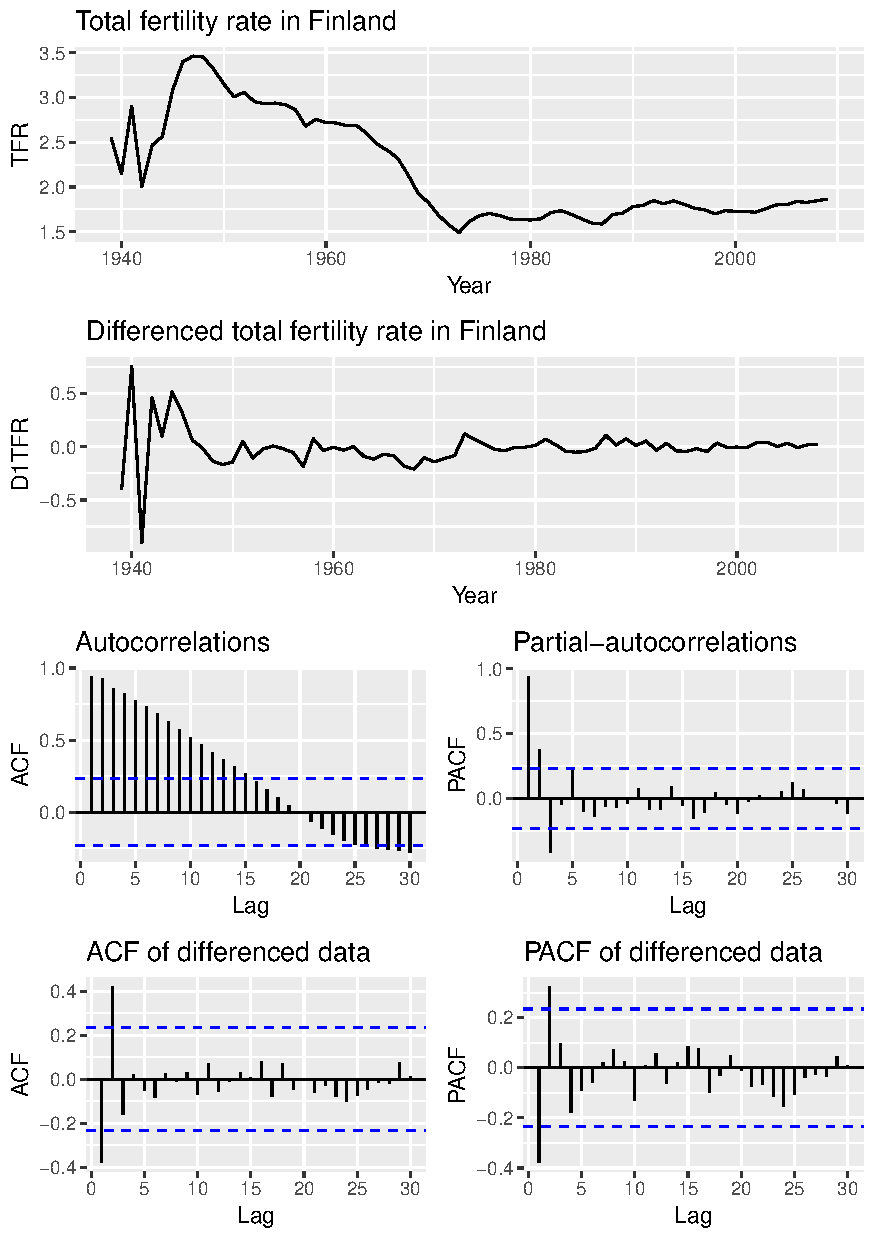
\includegraphics[height=0.85\textwidth, angle=-90]{ACFinland}
	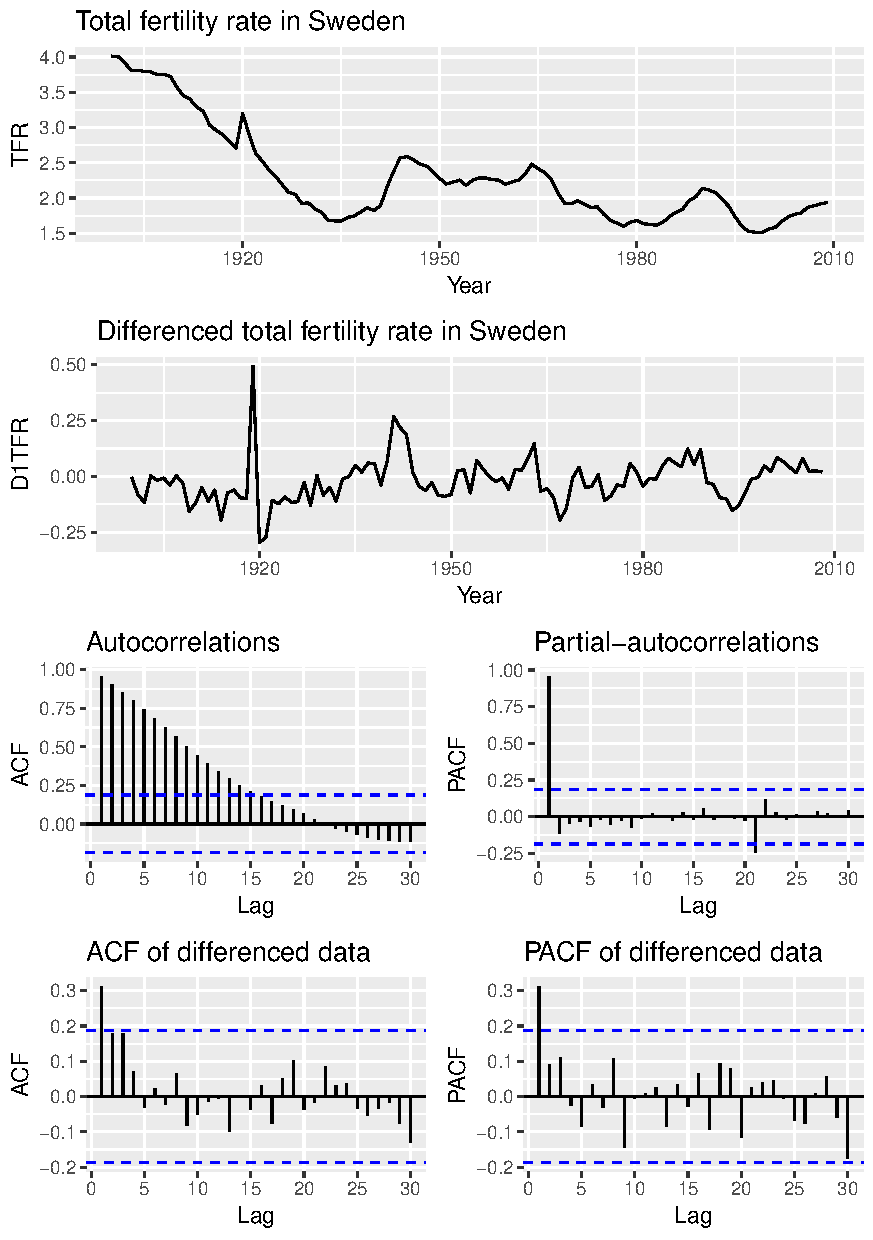
\includegraphics[height=0.85\textwidth, angle=-90]{ACSweden}
\end{figure}
\begin{figure}[h!]
	\centering
	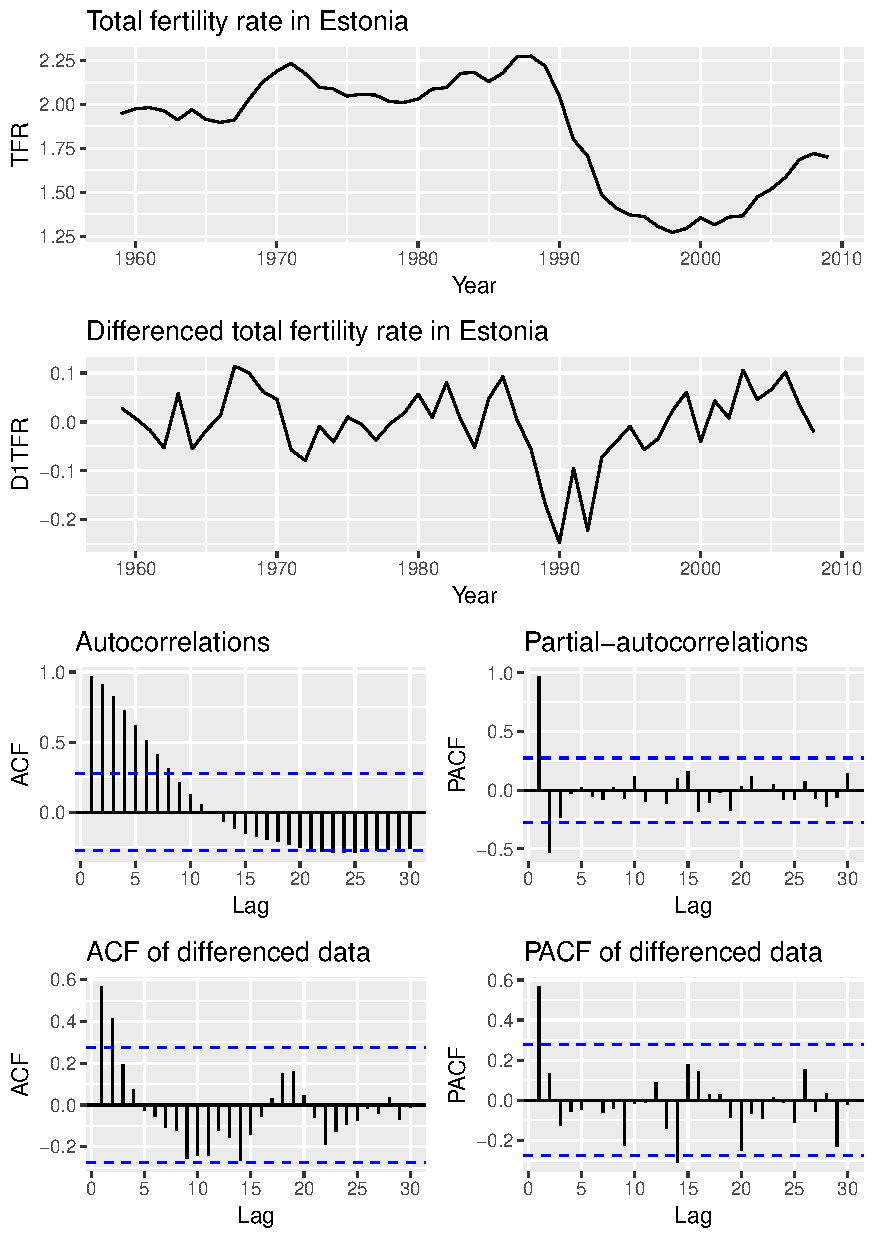
\includegraphics[height=0.85\textwidth, angle=-90]{ACEstonia}
	\includegraphics[height=0.85\textwidth, angle=-90]{"ACEngland and Wales".pdf}
\end{figure}
\begin{figure}[h!]
	\centering
	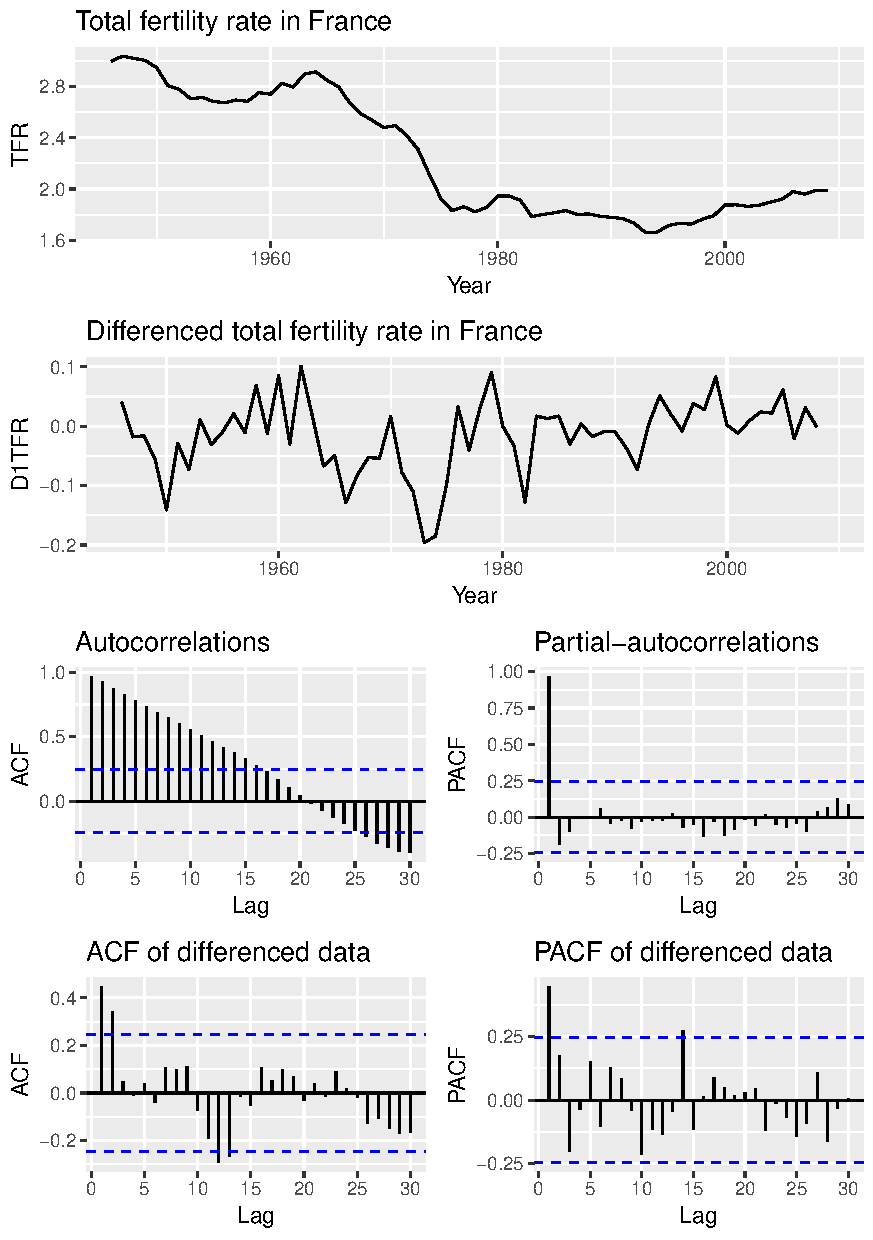
\includegraphics[height=0.85\textwidth, angle=-90]{ACFrance}
	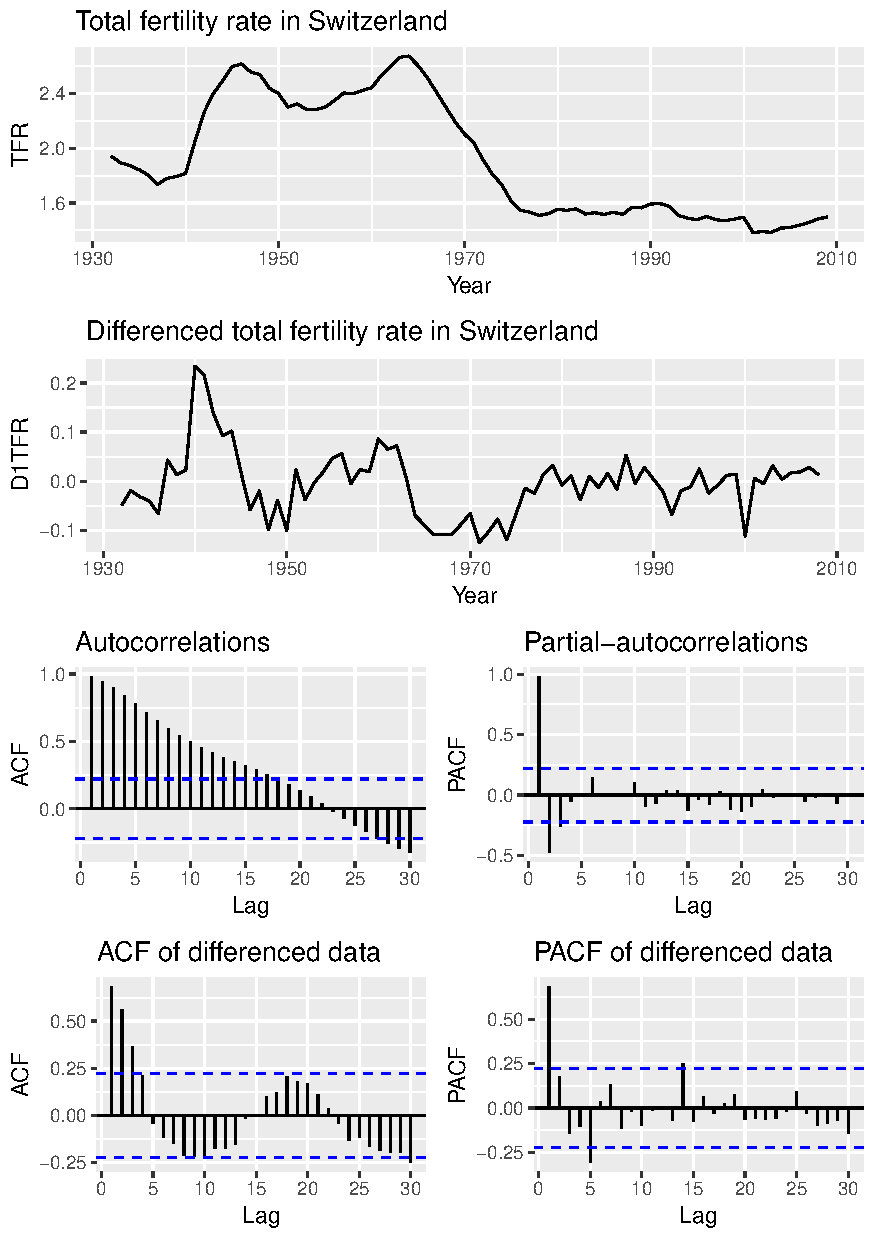
\includegraphics[height=0.85\textwidth, angle=-90]{ACSwitzerland}
\end{figure}
\begin{figure}[h!]
	\centering
	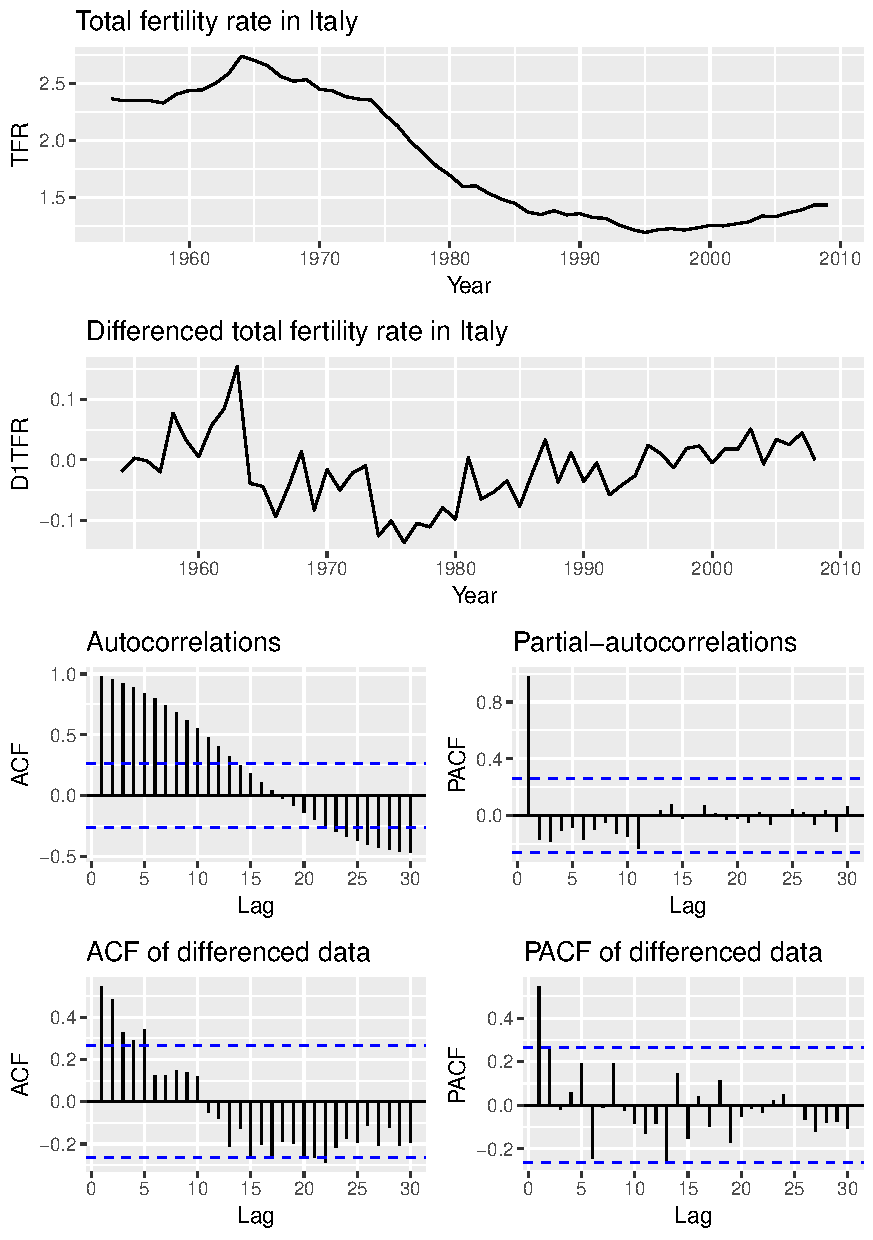
\includegraphics[height=0.85\textwidth, angle=-90]{ACItaly}
	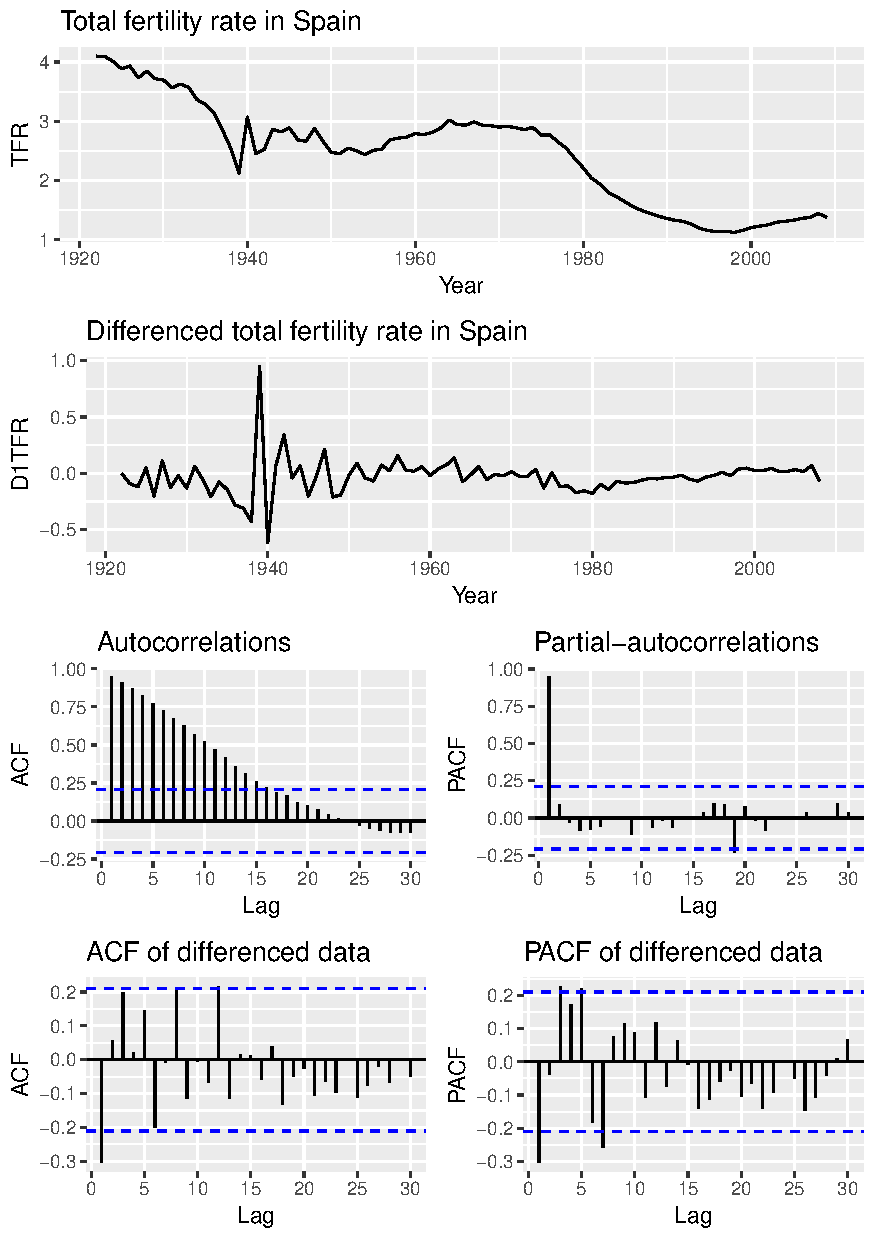
\includegraphics[height=0.85\textwidth, angle=-90]{ACSpain}
\end{figure}
\FloatBarrier
\newpage
\section{R-code}

\newpage
\begin{thebibliography}{3}
	\bibitem{web:TFR} \emph{Human Fertility Database}. Max Planck Institute for Demographic Research (Germany) and Vienna Institute of Demography (Austria). Available at \href{www.humanfertility.org}{www.humanfertility.org}. Accessed at 19.05.2018.
	
	\bibitem{web:fpp} Hyndman, R.J., \& Athanasopoulos, G. (2018). \emph{Forecasting: principles and practice}, 2nd edition, OTexts: Melbourne, Australia. \href{https://otexts.com/fpp2/}{OTexts.com/fpp2}. Accessed on 08.05.2019.
	
	\bibitem{art:hyndkhand} Hyndman, R. J., \& Khandakar, Y. (2008). \emph{Automatic time series forecasting: The forecast package for R.} Journal of Statistical Software, 27(1), 1-22.
\end{thebibliography}



\end{document}
